\chapter{Theory}

Developing for Android is done using the Java programming language, but requires the use of some additional classes and techniques to adapt the program for the operating system. Android also enables several data storage and retrieval options.

\section{Android architecture}

Developing applications for the Android platform is done using standard approaches of the Java programming language.

The Android operating system influences how applications are executed. Most operating systems on personals computers allow the user to run several applications concurrently in different windows, that can be viewed simultaneously. On the Android device, there is no native way to determine which applications are running. The hardware buttons on the device are used to either close applications or send them to the background. Since the user receives no feedback on what happened to the application, it is important to handle such events in a consistent manner, to avoid confusion.
 
Gaining access to the surface of an Android device requires an implementation of the Activity class. The first describing line in the Android API about activities is "An activity is a single, focused thing that the user can do" \citep{Android}. When compared to applications on a personal computer, the Activity can be seen as a window showing different user interface elements. To create an application that shows something to the user, an Activity must be implemented. If it is not important to display information to the user, the Service class may be used (a class designed for applications running in the background).

%-------------------
%- Image ACTIVITY DIAGRAM
%-------------------
\begin{figure}[here]
\begin{center}
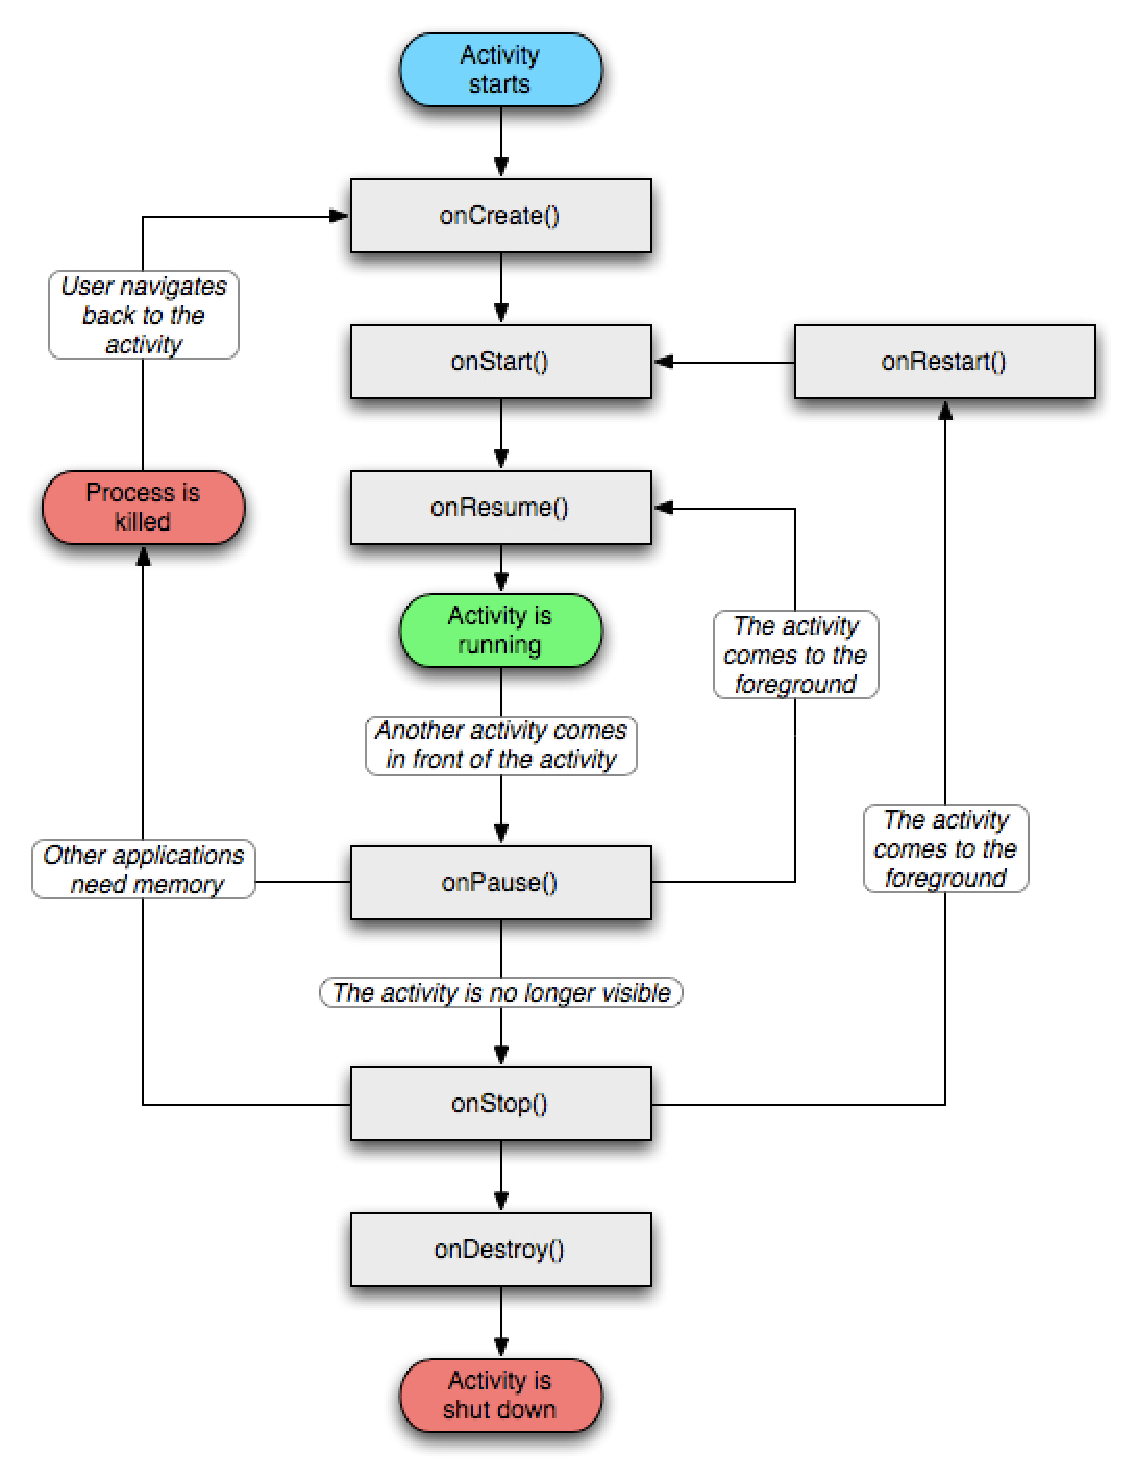
\includegraphics[scale=0.5]{pics/chapters/chapter2/activity_lifecycle2}
\end{center}
\caption{Life cycle of an Activity}
\label{fig:androidActivityLifeCycle}
\end{figure}
%-------------------------------

As can be seen in figure ~\ref{fig:androidActivityLifeCycle}; onCreate(), onStart() and onResume() are all invoked when an activity is first created. Several other methods are also invoked when the operating system needs to manage memory shortage. Once the activity is up and running, it is important to handle these methods correctly. For instance, if a lot of variables are instantiated in the onStart()-method memory leaks might occur, unless the variables are set to null in the onStop()-method. Memory leaks can cause the entire device to slow down, which can be very frustrating for the user.
 
The graphical layout of an activity consists of objects of the View class. Views can be defined either procedurally while creating the activity, or by accessing predefined layouts from XML-files. In Android applications, views are both responsible for drawing images to the screen and for taking care of events generated from user interaction. For instance, a button is a view that can register listeners for onClick-events. Similarly, events generated by the trackball, hardware buttons and touchscreen are also handled by views.

External resources are often used when developing for Android. Any type of file can be included to the binary files when building an application. If Eclipse is used to develop the application, a file called R.java is generated whenever the resource directory is updated. This file contains translations from integer resource pointers to variable names that are easier to understand. When the application is built, the resource files are compiled into binary files that load fast and efficiently. \citep{Android}
 
Accessing resources is done by invoking the method getResources() on the Context that is attached to the application. Context is an interface that is implemented by fundamental Android classes, such as Activity or Service. As stated in the Android API \citep{Android}, "It allows access to application-specific resources and classes.".

%----------------------------------------------------------
%----------------------------------------------------------
\subsection{Data storage}

The file system on Android devices differs from systems used on personal computers. On a personal computer, file system data files for one application can be read by any other application. On Android devices however data files created by one application is only readable to that application. Android has four different solutions to store and receive data; preferences, files, databases and network. \citep{Android} 

The preferences solution uses key-value pairs to write simple data types. It can be used for texts that should be loaded at the start of an application, or for settings that the user wants to save until next time he starts the application. This data is a lightweight method of writing and retrieving data, and is therefore recommended to use for simple data types. \citep{Android}

Another way to manage data storage is to use files. This is a basic way to handle data on the mobile phone's memory card, where files are created, written to and read from. \citep{Android} 

Android provides the ability to use databases for data storage. The type of database available on a Android device is SQLite. \citep{Android} SQLite is a lightweight database engine, built to suit devices with limited memory. It reads and writes to files on the device's file system. "A complete SQL database with multiple tables, indices, triggers, and views, is contained in a single disk file." \citep{SQLite}

As long as the phone is connected to the Internet, either via 3G or via a wireless network, it is possible to use the network connection to send and receive data. \citep{Android}
%----------------------------------------------------------
%----------------------------------------------------------
\subsection{Graphics}

There are three approaches to handling graphics when working with Android. The first approach uses predefined layouts in XML-files. The other two approaches involve the Java class Canvas or the cross-language standard specification OpenGL. The Canvas class provides simple tools like rectangles, color filters and bitmaps that let you draw pictures on the screen. It works in a similar way as layers: the last object that is drawn on the canvas will be drawn on top of anything that was drawn earlier. Canvas only supports two axes, x- and y-coordinates compared to OpenGL that has full support for programming 3D graphics.

For each activity using a predefined layout, there has to be an XML-file describing that layout. There is a built-in XML-editor in the Android Software Development Kit for Eclipse that can be used to create these layouts. The editor shows a preview of the window that will be shown on the screen of the device (figure ~\ref{fig:xmlEditor}). All the graphics are put inside that window. The editor is very easy to use as it uses the drag-and-drop concept. 

There are several layout options, that govern how elements will be placed, such as GridView, ListView and LinearLayout to choose between or combine. There are also several view options such as normal View, Button, Checkbox, TextView and many more. Items are dragged and dropped to their correct positions. There is also a property window for every item, that gives access to customizing that particular item in the layout.

%-------------------------
%- IMAGE XML Editor
%-------------------------
\begin{figure}[here]
\begin{center}
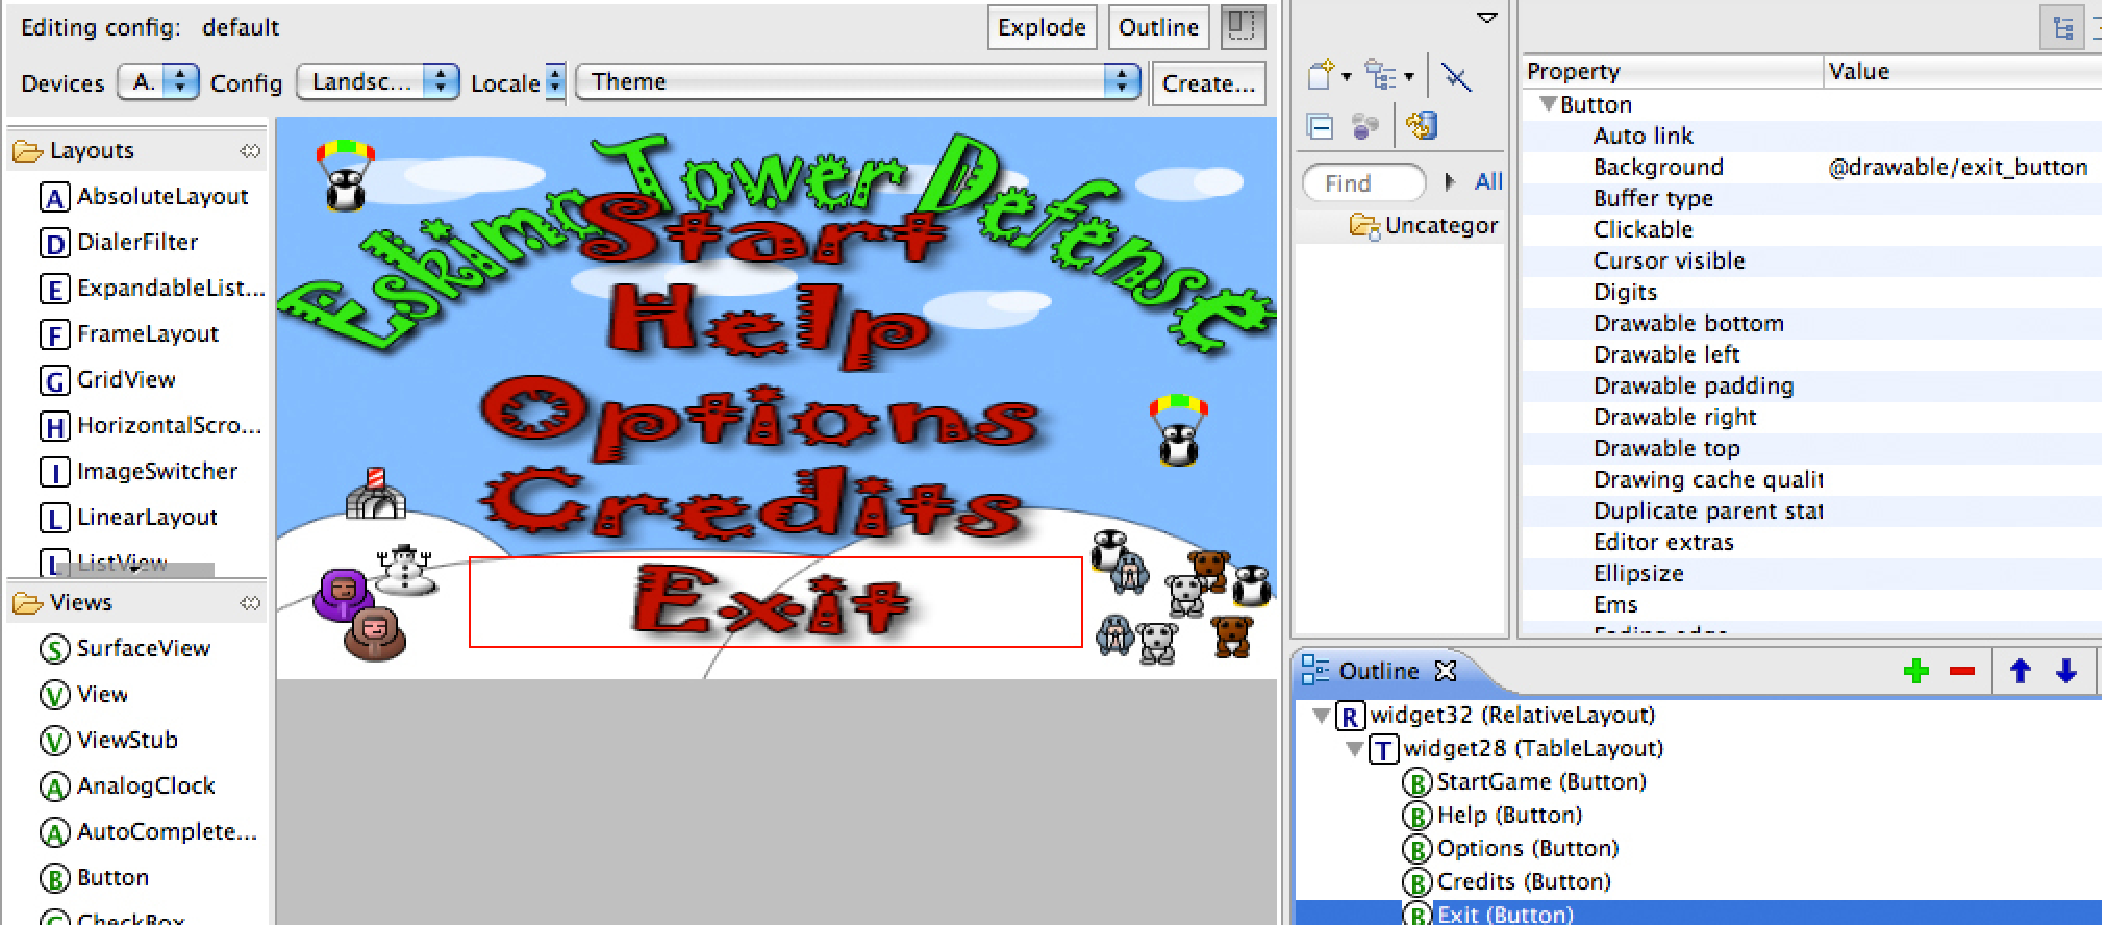
\includegraphics[scale=0.3]{pics/chapters/chapter2/xmleditor}
\end{center}

\caption{The XML editor in Eclipse}
\label{fig:xmlEditor}

\end{figure}
%-------------------------

%----------------------------------------------------------
%----------------------------------------------------------
\subsection{Sound}

The Android operating system is able to provide playback of different media files. A list of all supported media formats is published in the Android API \citep{Android}. When considering sound files in particular, all of the major sound formats (MP3, MIDI, WAVE, Ogg Vorbis and more) are supported. Unless playing sounds is the main purpose of the application, it is desirable to use files that are small and therefore require less memory. 

Sound implementation in Android applications is done by utilizing the classes MediaPlayer and SoundPool. The SoundPool class should be used for small sounds, that are likely to be repeated a lot. Sounds added to a SoundPool are decoded by a MediaPlayer and stored as raw bitstreams. Not having to decode sound files every time they are played reduces the risk of experiencing performance issues due to heavy CPU load. MediaPlayer is better used for long sound files, such as background music. \citep{Android}
%----------------------------------------------------------